\chapter{Analisis}
\label{chap:analisis}

\section{Analisis Portal Akademik Mahasiswa}
Portal Akademik Mahasiswa merupakan sebuah situs jaringan yang diperuntukan bagi mahasiswa dalam rangka mendapatkan informasi kegiatan akademik\cite{BTI:2012}. Mahasiswa dapat mengakses Portal Akademik Mahasiswa melalui URL \url{https://studentportal.unpar.ac.id/}. Untuk mengakses Portal Akademik Mahasiswa, mahasiswa harus \textit{login} menggunakan akun email \textit{student}. Halaman \textit{login} Student Portal UNPAR terintegrasi dengan CAS (\textit{Central Authentication Service}) UNPAR\footnote{\url{https://cas.unpar.ac.id}}.

\begin{figure}[H]
	\centering
	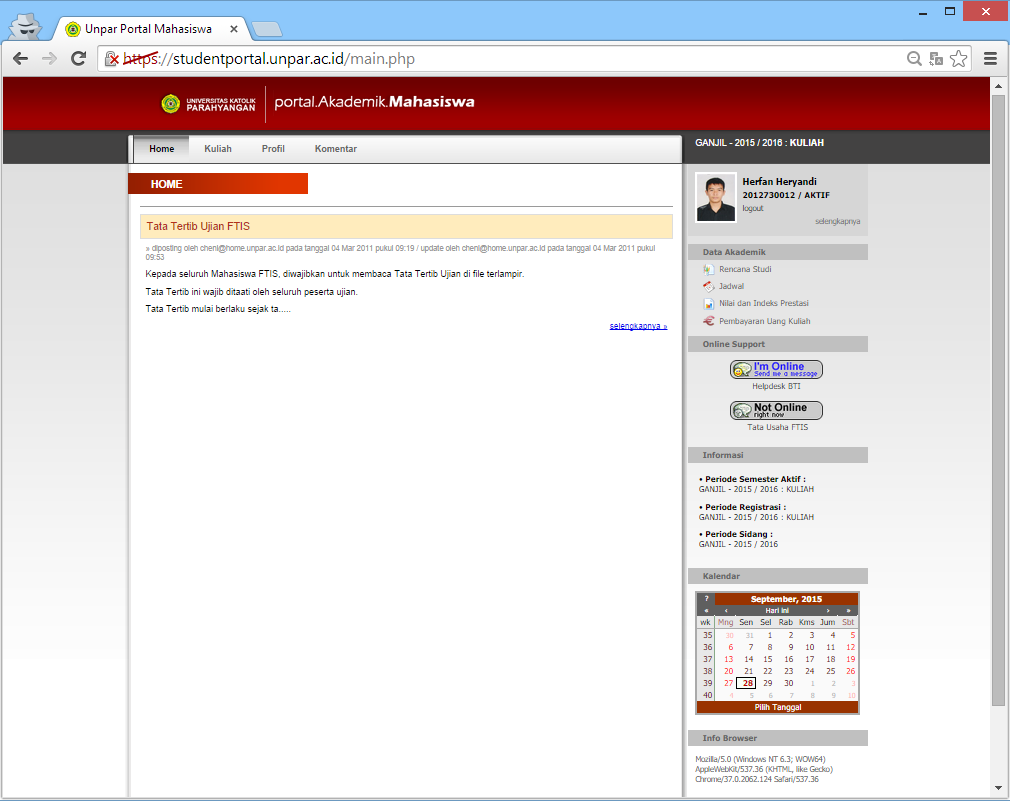
\includegraphics[scale=0.5]{Gambar/pam-home}
	\caption{Halaman Utama Portal Akademik Mahasiswa} 
	\label{fig:3_pam_home}
\end{figure}

Pada halaman utama Portal Akademik Mahasiswa (gambar \ref{fig:3_pam_home}), terdapat beberapa bagian yaitu:
\begin{enumerate}
	\item Menu Atas\\
	Menu ini berfungsi sebagai menu pendukung yang terdiri dari : 
	\begin{itemize}
		\item \textbf{Home}, menampilkan informasi atau pengumuman yang dikeluarkan oleh fakultas masing-masing (Gambar \ref{fig:3_pam_atas_home}). 
		
		\begin{figure}[H]
			\centering
			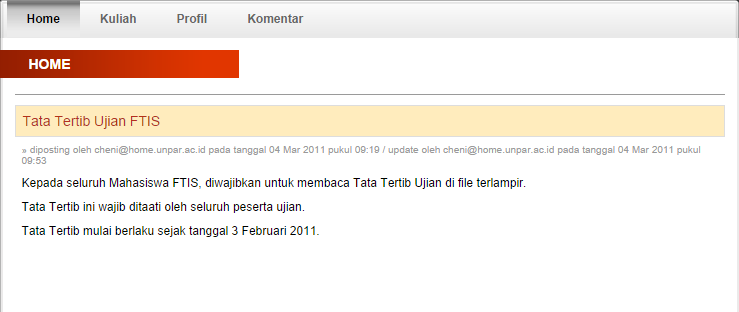
\includegraphics[scale=0.5]{Gambar/pam-atas-home}
			\caption{Menu Atas Home} 
			\label{fig:3_pam_atas_home}
		\end{figure}
		
		\item \textbf{Kuliah}, menampilkan pengumuman per mata kuliah sesuai dengan mata kuliah dan kelas yang diambil oleh masing-masing mahasiswa (Gambar \ref{fig:3_pam_atas_kuliah}).  
		
		\begin{figure}[H]
			\centering
			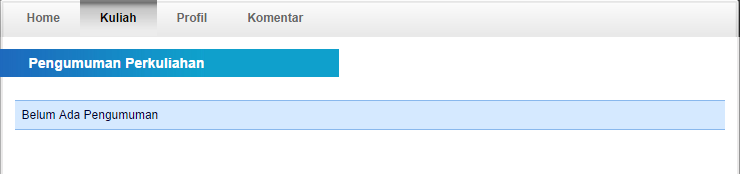
\includegraphics[scale=0.5]{Gambar/pam-atas-kuliah}
			\caption{Menu Atas Kuliah} 
			\label{fig:3_pam_atas_kuliah}
		\end{figure}
		
		\item \textbf{Profil}, berisi tentang data diri masing-masing mahasiswa (Gambar \ref{fig:3_pam_atas_profil}). 
		
		\begin{figure}[H]
			\centering
			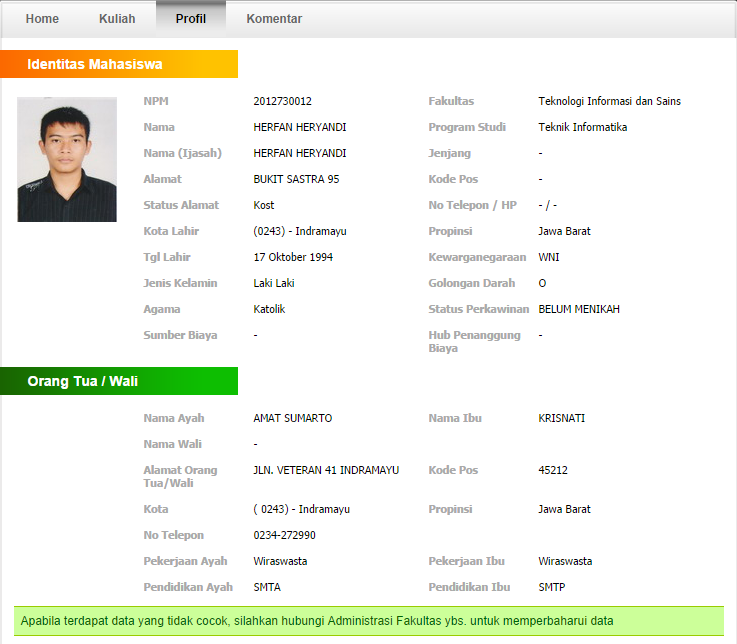
\includegraphics[scale=0.5]{Gambar/pam-atas-profil}
			\caption{Menu Atas Profil} 
			\label{fig:3_pam_atas_profil}
		\end{figure}
		
		\item \textbf{Komentar}, berisi komentar, saran, dan kritik dari mahasiswa (Gambar \ref{fig:3_pam_atas_komentar}).
		
		\begin{figure}[H]
			\centering
			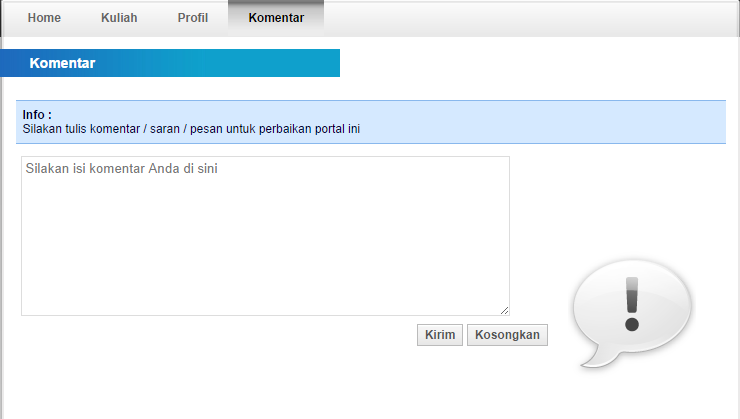
\includegraphics[scale=0.5]{Gambar/pam-atas-komentar}
			\caption{Menu Atas Komentar} 
			\label{fig:3_pam_atas_komentar}
		\end{figure}

	\end{itemize}
	
	\item Identitas Portal \\
	Bagian ini menampilkan identitas pengguna portal. Tampilan identitas ini dapat ditampilkan lengkap dengan melakukan klik pada \textit{link} ``selengkapnya'' atau ditampilkan minimal dengan klik \textit{link} ``tutup''. Identitas yang ditampilkan adalah nama, Nomor Pokok Mahasiswa (NPM), status keaktifan, pas foto, email, dosen wali, program studi, dan fakultas seperti yang terlihat pada gambar \ref{fig:3_pam_identitas}.   
	\begin{figure}[H]
			\centering
			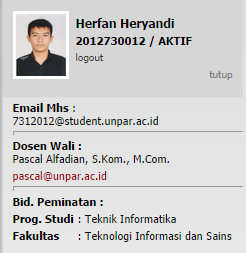
\includegraphics[scale=0.75]{Gambar/pam-identitas}
			\caption{Identitas Portal} 
			\label{fig:3_pam_identitas}
		\end{figure}
		
	\item Menu Utama\\
	Bagian ini memuat fitur utama Portal Akademik Mahasiswa mengenai data akademik (gambar \ref{fig:3_pam_utama}) yang terdiri dari:
		\begin{figure}[H]
			\centering
			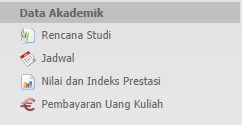
\includegraphics[scale=0.75]{Gambar/pam-utama}
			\caption{Menu Utama} 
			\label{fig:3_pam_utama}
		\end{figure}
	\begin{itemize}
	
		\item \textbf{Rencana Studi}\\
		Menu Rencana Studi terdiri dari submenu: 
		\begin{itemize}
			\item Registrasi (FRS/PRS)\\
			Digunakan sebagai formulir pengisian rencana studi awal (FRS) dan perubahan rencana studi (PRS) (Gambar \ref{fig:3_pam_utama_registrasi}). 			%belum relevan
			\begin{figure}[H]
				\centering
				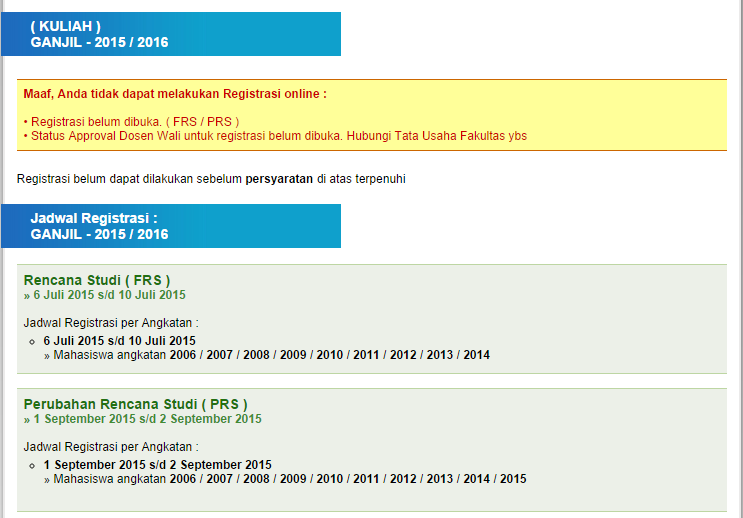
\includegraphics[scale=0.5]{Gambar/pam-utama-rencanastudi}
				\caption{Tampilan Registrasi FRS/PRS} 
				\label{fig:3_pam_utama_registrasi}
			\end{figure}
			
			\item Kartu Rencana Studi \\
			Menampilkan informasi mata kuliah yang telah diambil melalui submenu Registrasi (Gambar \ref{fig:3_pam_utama_krs}). Kartu Rencana Studi juga dapat dicetak melalui submenu ini. 
			\begin{figure}[H]
				\centering
				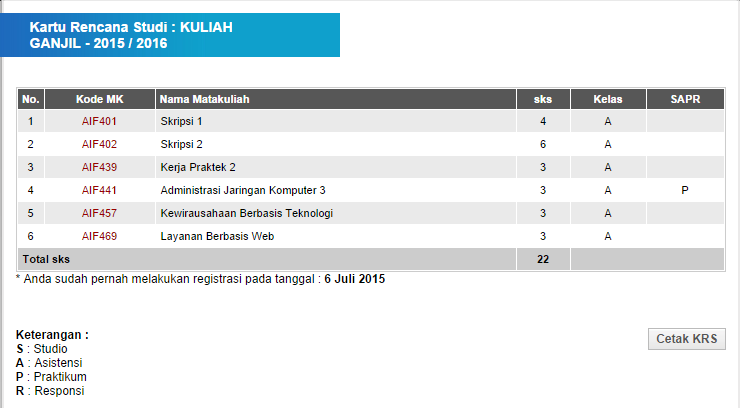
\includegraphics[scale=0.5]{Gambar/pam-utama-krs}
				\caption{Tampilan Kartu Rencana Studi} 
				\label{fig:3_pam_utama_krs}
			\end{figure}
			
			\item Pindah Kelas MKU \\
			Mahasiswa dapat memilih kelas yang masih tersedia di kolom Jadwal Baru dan menekan tombol ``Simpan'' untuk setiap kelas yang diubah (Gambar \ref{fig:3_pam_utama_pindahmku}). 
			%belum relevan
			\begin{figure}[H]
				\centering
				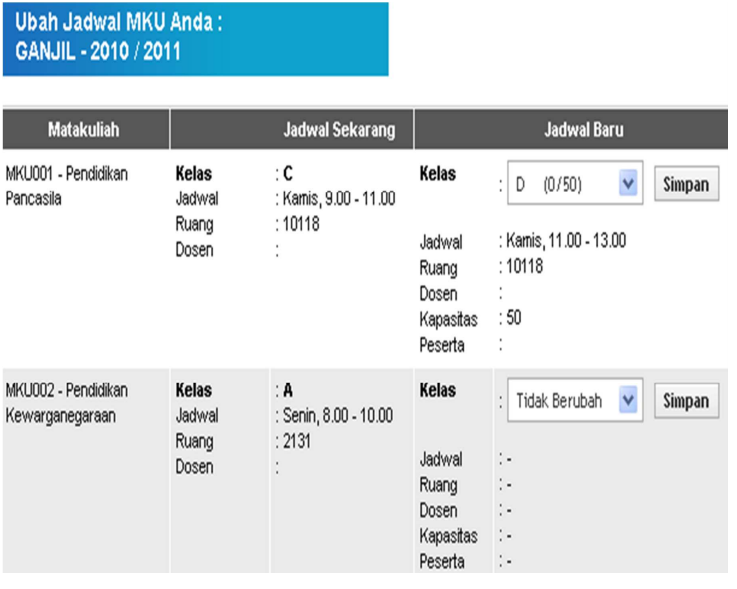
\includegraphics[scale=0.5]{Gambar/pam-utama-pindahmku}
				\caption{Tampilan Pindah Kelas MKU} 
				\label{fig:3_pam_utama_pindahmku}
			\end{figure}

		\end{itemize}
		
		\item \textbf{ Jadwal}\\
		Menu Jadwal terdiri dari submenu: 
		\begin{itemize}
			\item Kuliah, UTS, dan UAS \\
			Submenu ini berisi tentang jadwal kuliah, UTS dan UAS yang dapat disusun per semester (Gambar \ref{fig:3_pam_utama_jadwal}). 
			\begin{figure}[H]
				\centering
				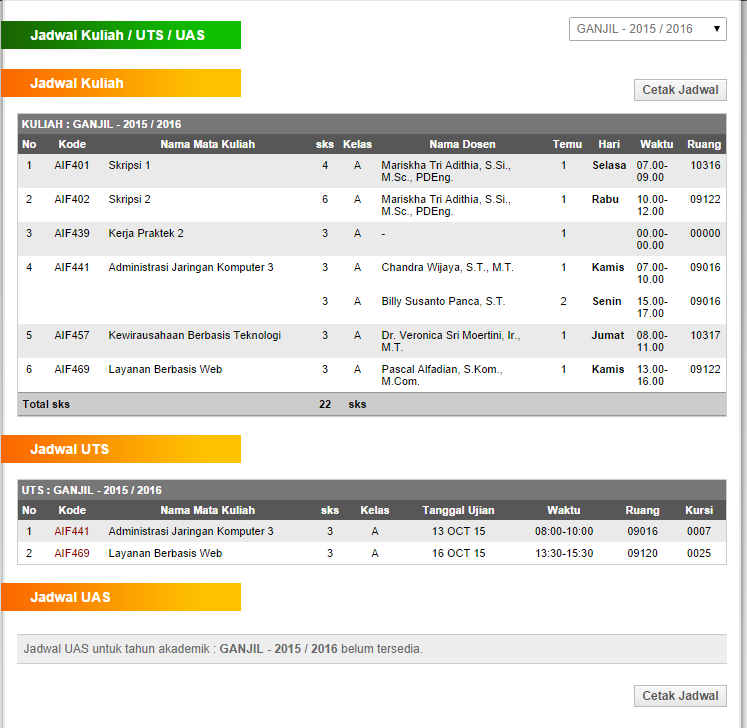
\includegraphics[scale=0.5]{Gambar/pam-utama-jadwal}
				\caption{Tampilan Jadwal Kuliah, UTS, dan UAS} 
				\label{fig:3_pam_utama_jadwal}
			\end{figure}
			
			\item MKU \\
			Submenu ini menampilkan seluruh jadwal Mata Kuliah Umum (MKU) yang memberikan informasi tentang kelas-kelas yang dibuka oleh Pusat Kajian Humaniora (PKH) (Gambar \ref{fig:3_pam_utama_jadwalmku}). 
			\begin{figure}[H]
				\centering
				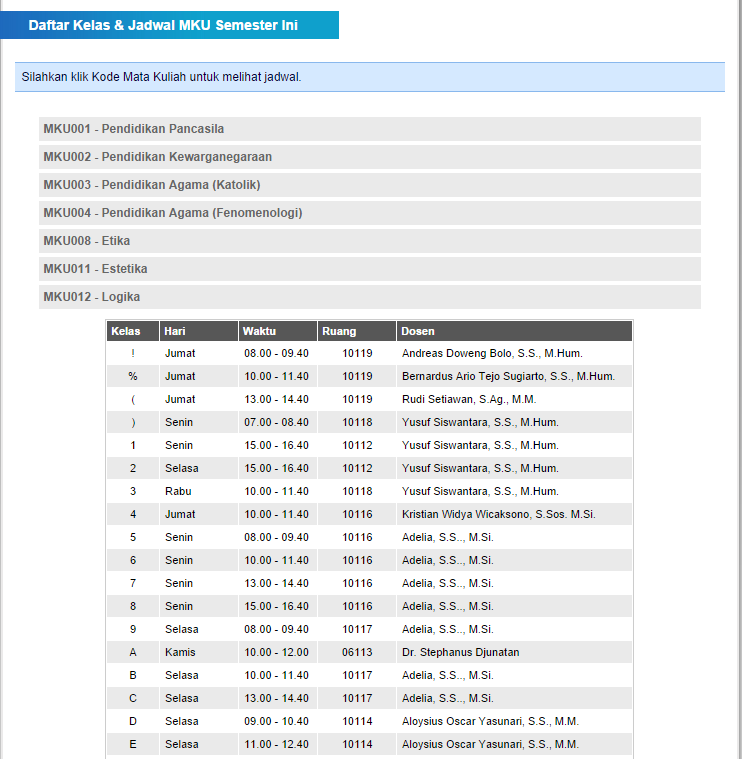
\includegraphics[scale=0.5]{Gambar/pam-utama-jadwalmku}
				\caption{Tampilan Jadwal MKU} 
				\label{fig:3_pam_utama_jadwalmku}
			\end{figure}
			
			\item Seluruh Fakultas \\
			Fitur ini memberikan informasi mengenai jadwal-jadwal yang ada di seluruh fakultas (Gambar \ref{fig:3_pam_utama_jadwalall}).
			\begin{figure}[H]
				\centering
				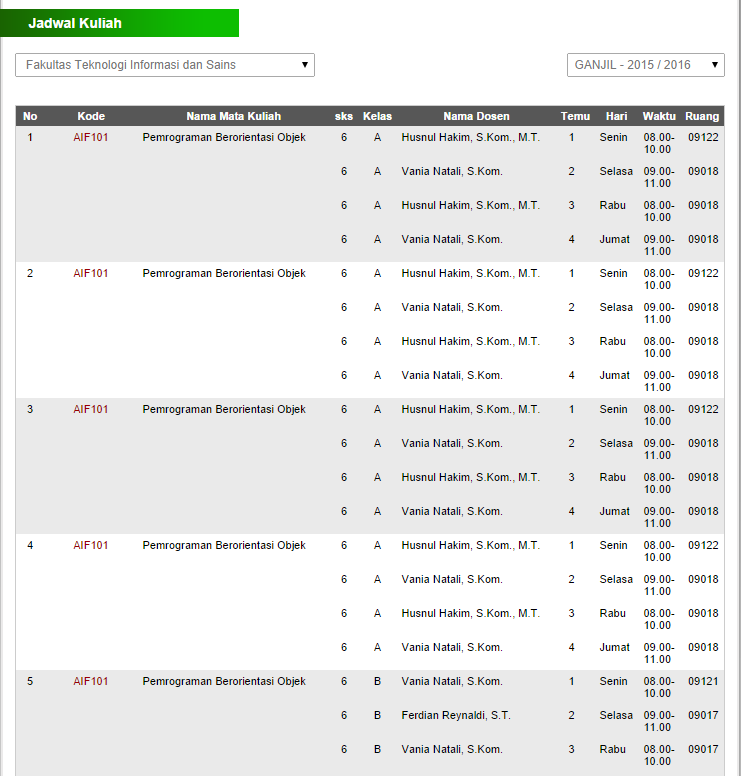
\includegraphics[scale=0.5]{Gambar/pam-utama-jadwalall}
				\caption{Tampilan Jadwal Seluruh Fakultas} 
				\label{fig:3_pam_utama_jadwalall}
			\end{figure}
		\end{itemize}
		
		\item \textbf{Nilai dan Indeks Prestasi}\\
		Menu Nilai dan Indeks Prestasi terdiri dari submenu: 
		\begin{itemize}
			\item Riwayat per Semester \\
			Submenu ini menampilkan informasi nilai per semester. Mahasiswa dapat melihat nilai sesuai dengan semester yang dipilih atau bisa memilih
pilihan ``Seluruh Tahun Akademik'' untuk melihat seluruh nilai berdasarkan semester (Gambar \ref{fig:3_pam_utama_nilai}).
			\begin{figure}[H]
				\centering
				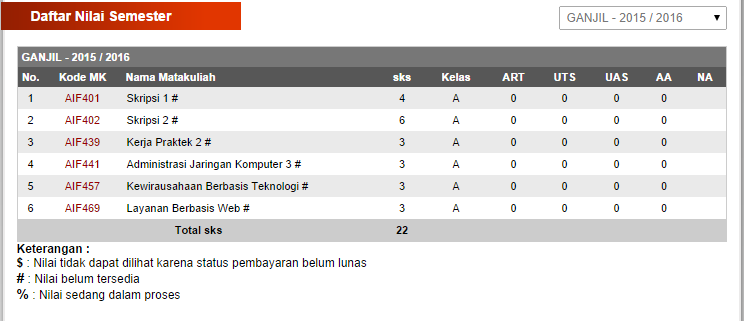
\includegraphics[scale=0.5]{Gambar/pam-utama-nilai}
				\caption{Tampilan Riwayat Per Semester} 
				\label{fig:3_pam_utama_nilai}
			\end{figure}
			
			\item Daftar Perkembangan Studi \\
			Seluruh riwayat mata kuliah dan nilai yang pernah ditempuh ditampilkan di submenu ini (Gambar \ref{fig:3_pam_utama_dps}). Pada bagian bawah halaman, terdapat statistik nilai dan indeks prestasi (Gambar \ref{fig:3_pam_utama_dpsstat}). 
			\begin{figure}[H]
				\centering
				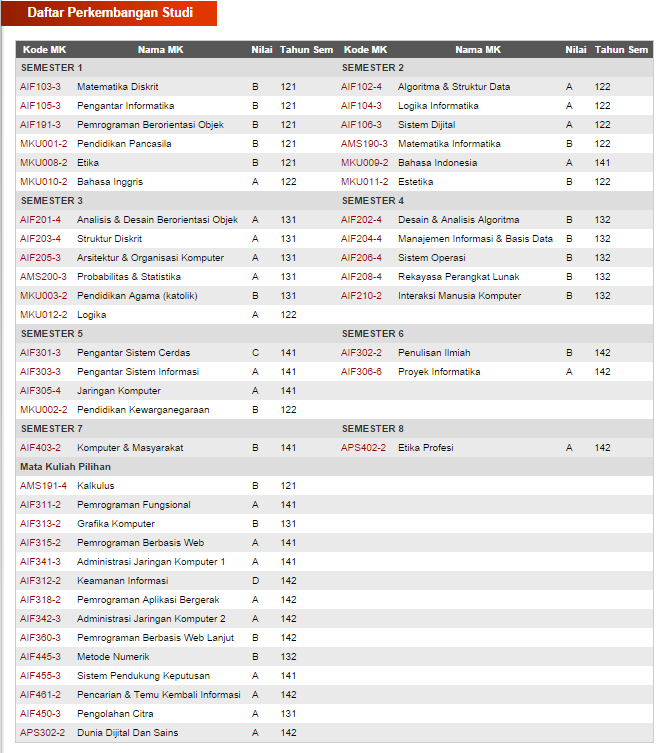
\includegraphics[scale=0.5]{Gambar/pam-utama-dps}
				\caption{Tampilan Daftar Perkembangan Studi} 
				\label{fig:3_pam_utama_dps}
			\end{figure}
			
			\begin{figure}[H]
				\centering
				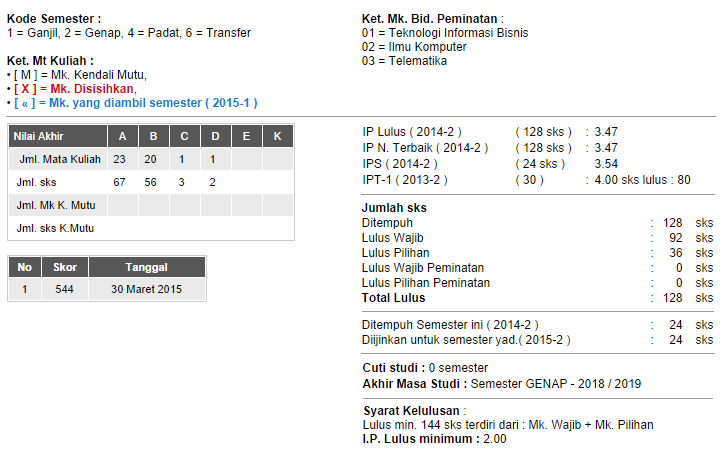
\includegraphics[scale=0.5]{Gambar/pam-utama-dpsstat}
				\caption{Tampilan Statistik Nilai dan IP} 
				\label{fig:3_pam_utama_dpsstat}
			\end{figure}
			
			\item Riwayat Indeks Prestasi \\
			Menampilkan daftar riwayat indeks prestasi semester dan kumulatif setiap semester. Tampilan ini juga dilengkapi dengan grafik perkembangan (Gambar \ref{fig:3_pam_utama_ip}). 
			\begin{figure}[H]
				\centering
				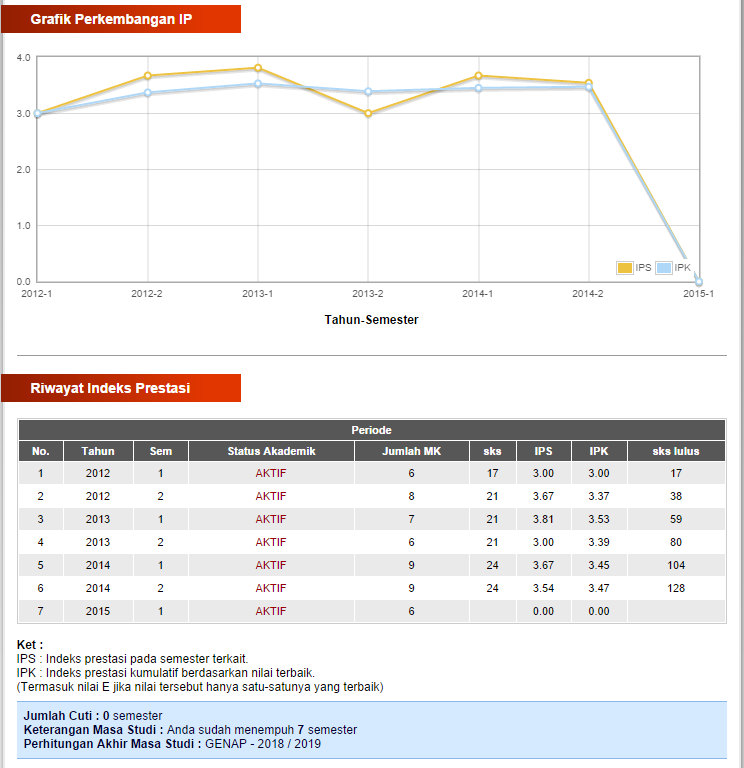
\includegraphics[scale=0.5]{Gambar/pam-utama-ip}
				\caption{Tampilan Riwayat Indeks Prestasi} 
				\label{fig:3_pam_utama_ip}
			\end{figure}
			
			\item TOEFL \\
			Menampilkan daftar riwayat skor \textit{Test of English as Foreign Language} (TOEFL) yang pernah ditempuh (Gambar \ref{fig:3_pam_utama_toefl}). Mahasiswa diwajibkan untuk menempuh TOEFL dengan skor minimal 500.
			
			\begin{figure}[H]
				\centering
				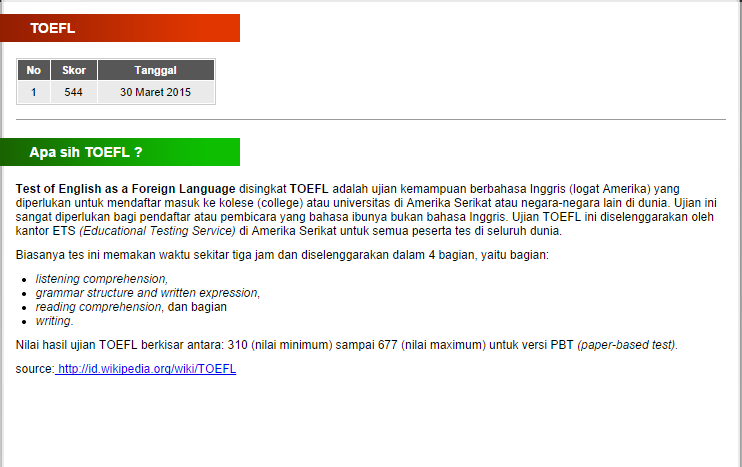
\includegraphics[scale=0.5]{Gambar/pam-utama-toefl}
				\caption{Tampilan TOEFL} 
				\label{fig:3_pam_utama_toefl}
			\end{figure}
		\end{itemize}
		
		\item \textbf{Pembayaran Uang Kuliah}\\
		Menu ini berfungsi untuk melihat data tagihan pembayaran uang kuliah serta cara-cara pembayarannya (Gambar \ref{fig:3_pam_utama_pembayaran}).
		\begin{figure}[H]
				\centering
				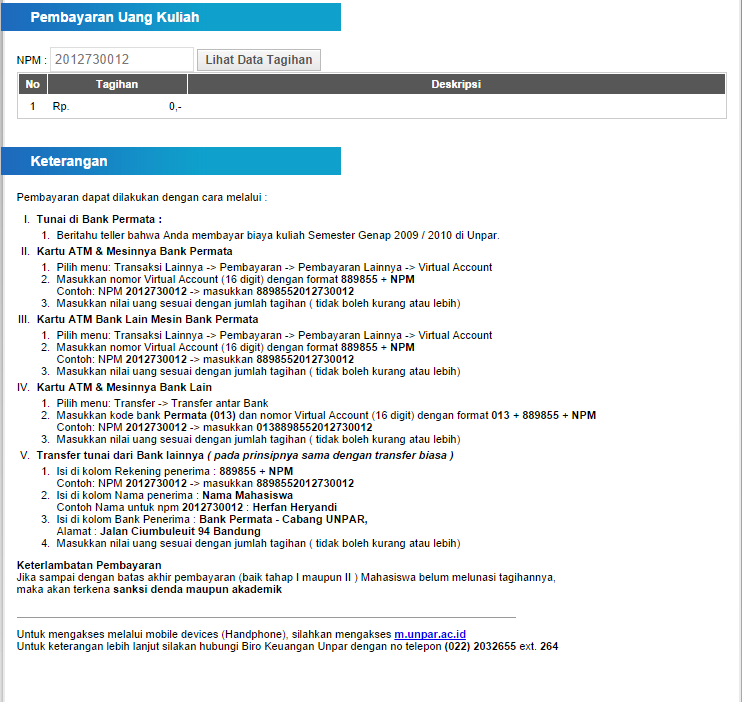
\includegraphics[scale=0.5]{Gambar/pam-utama-pembayaran}
				\caption{Tampilan Pembayaran Uang Kuliah} 
				\label{fig:3_pam_utama_pembayaran}
			\end{figure}
		\end{itemize}
		
	\item \textbf{Informasi}\\
		Bagian ini menampilkan informasi tentang periode-periode yang sedang aktif (Gambar \ref{fig:3_pam_utama_informasi}). Sebagai contoh jika ``Periode Registrasi'' diklik maka akan muncul \textit{pop up} seperti pada gambar \ref{fig:3_pam_utama_informasipop}.
			\begin{figure}[H]
				\centering
				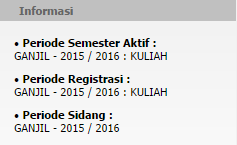
\includegraphics[scale=0.75]{Gambar/pam-utama-informasi}
				\caption{Tampilan Informasi} 
				\label{fig:3_pam_utama_informasi}
			\end{figure}
			
			\begin{figure}[H]
				\centering
				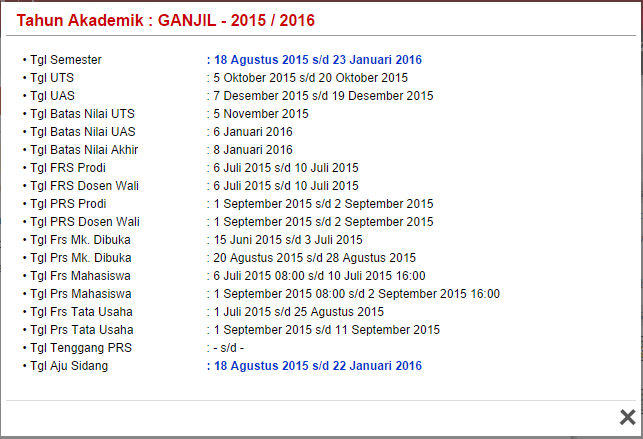
\includegraphics[scale=0.5]{Gambar/pam-utama-infopop}
				\caption{Tampilan \textit{Pop Up} Informasi} 
				\label{fig:3_pam_utama_informasipop}
			\end{figure}
		
	\item \textbf{Kalender}\\
		Bagian ini menampilkan kalender masehi (Gambar \ref{fig:3_pam_utama_kalender}).
		\begin{figure}[H]
				\centering
				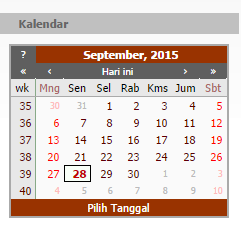
\includegraphics[scale=0.75]{Gambar/pam-utama-kalender}
				\caption{Tampilan Kalender} 
				\label{fig:3_pam_utama_kalender}
			\end{figure}
		
	\item \textbf{Info Browser}\\
		Bagian ini menampilkan informasi tentang internet \textit{browser} yang digunakan pada saat membuka Portal Akademik Mahasiswa (Gambar \ref{fig:3_pam_utama_infobrowser}). 
		\begin{figure}[H]
				\centering
				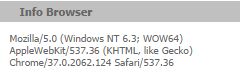
\includegraphics[scale=0.75]{Gambar/pam-utama-infobrowser}
				\caption{Tampilan Info Browser} 
				\label{fig:3_pam_utama_infobrowser}
			\end{figure}
\end{enumerate}

\section{Analisis Kebutuhan IT Student Portal}
Dalam menganalisis kebutuhan IT Student Portal, penulis melakukan wawancara dengan 18 mahasiswa Program Studi Teknik Informatika UNPAR. Kriteria dari 18 mahasiswa tersebut yaitu lipsum. Setelah melakukan wawancara, penulis memperoleh fitur-fitur yang diinginkan mahasiswa antara lain:
\begin{enumerate}
	\item Prasyarat mata kuliah
	\item Status perkuliahan
	\item Perubahan IPS dan IPK berdasarkan riwayat nilai
	\item Jadwal kuliah yang tersusun
	\item Kalender akademik
	\item Rincian pembayaran
	\item Rincian mata kuliah
	\item Tampilan situs web sama di sistem operasi manapun 
	\item Kontak dosen
	\item Pohon kurikulum
	\item Pemberitahuan
	\item \textit{Chatting}
	\item Unggah \textit{Curriculum Vitae}
\end{enumerate}

Fitur-fitur yang akan dipilih untuk diimplementasikan harus memenuhi kriteria:
\begin{itemize}
	\item Data yang dibutuhkan dapat diambil dari Portal Akademik Mahasiwa
	\item Fitur tidak tersedia di Portal Akademik Mahasiswa
	\item Fitur mendukung fungsi Portal Akademik Mahasiswa sebagai sumber informasi akademik
\end{itemize}

Berdasarkan kriteria di atas dan batas waktu pembangunan aplikasi, maka akan dipilih fitur-fitur sebagai berikut:
\begin{enumerate}
	\item Prasyarat mata kuliah
	\item Susunan jadwal yang terurut 
	\item Tampilan \textit{desktop} pada sistem operasi selain Windows
\end{enumerate}


\section{Analisis Komunikasi Portal Akademik Mahasiswa untuk Fitur IT Student Portal}
Untuk memenuhi fitur IT Student Portal, penulis menganalisis komunikasi Portal Akademik Mahasiswa ke dalam beberapa kasus yang akan dijelaskan pada subbab-subbab berikut.

\subsection{Kasus \textit{Login}}
Di Portal Akademik Mahasiswa, mahasiswa dapat login dengan mengakses \url{https://studentportal.unpar.ac.id/} dan mengklik tombol \texttt{input#submit.login-button} (Gambar \ref{}). Saat tombol tersebut ditekan, mahasiswa akan dibawa ke halaman \texttt{index.login.submit.php} dengan form data berisi \texttt{Submit: Login}. Lalu mahasiswa akan diarahkan ke \url{https://cas.unpar.ac.id/login?service=https\%3A\%2F\%2Fstudentportal.unpar.ac.id\%2Fhome\%2Findex.login.submit.php}. Di sana, mahasiswa akan ditampilkan halaman \textit{login} CAS UNPAR di mana mahasiswa diminta mengisi ``Username'' pada \textit{textfield} \texttt{input#username.required} dan mengisi ``Password'' pada \textit{password field} \texttt{input#password.required}. Setelah itu mahasiswa harus menekan tombol \texttt{input.btn-submit}. Data tersebut akan dikirimkan ke URL \url{} yang mengandung form data seperti pada gambar \ref{}. Jika berhasil, akan dilakukan pengalihan ke \url{https://studentportal.unpar.ac.id/main.php} dengan cookie.

\subsection{Kasus Nilai}
Di halaman utama Portal Akademik Mahasiswa, mahasiswa dapat melihat nilai dengan mengklik \texttt{a.first-line-menu} dengan teks ``Nilai dan Indeks Prestasi'' kemudian akan muncul \texttt{ul.hidden}. Dalam \textit{list} tersebut, mahasiswa harus mengklik \texttt{a} dengan teks ``Riwayat Per Semester''. Mahasiswa akan diarahkan ke \url{https://studentportal.unpar.ac.id/includes/nilai.daftar_sem.php} yang menampilkan nilai semester terkini. Untuk melihat riwayat nilai seluruh semester, mahasiswa harus mengklik \textit{combo box} \texttt{select#tahun_akd_sec} kemudian memilih \texttt{option} ``Seluruh Tahun Akademik''. Mahasiswa akan diarahkan ke \url{https://studentportal.unpar.ac.id/includes/nilai.sem.php} yang mengandung form data seperti pada gambar \ref{}.

\subsection{Kasus Jadwal}
Mahasiswa dapat melihat nilai dengan mengklik \texttt{a.first-line-menu} dengan teks ``Jadwal'' kemudian akan muncul \texttt{ul.hidden}. Dalam \textit{list} tersebut, mahasiswa harus mengklik \texttt{a} dengan teks ``Kuliah, UTS dan UAS''. Kemudian mahasiswa diarahkan ke \url{https://studentportal.unpar.ac.id/includes/jadwal.aktif.php} yang menampilkan jadwal kuliah, UTS, dan UAS semester terkini. Mahasiswa juga dapat melihat jadwal semester sebelumnya dengan mengklik \textit{combo box} \texttt{select#tahun_akd_sec} kemudian memilih \texttt{option} semester yang diinginkan.

Selain jadwal kuliah, UTS, dan UAS, mahasiswa juga dapat melihat jadwal seluruh fakultas. Dengan mengklik \texttt{a} dengan teks ``Seluruh Fakultas'' pada \textit{list} \texttt{ul.hidden}, mahasiswa akan diarahkan ke \url{https://studentportal.unpar.ac.id/includes/jadwal.all.php}. Halaman tersebut menampilkan jadwal seluruh fakultas semester terkini. Mahasiswa dapat melihat jadwal semester sebelumnya dengan mengklik \textit{combo box} \texttt{select#tahun_akd_sec} kemudian memilih \texttt{option} semester yang diinginkan dan dapat melihat jadwal fakultas lainnya dengan mengklik \textit{combo box} \texttt{select#jadwal_all_ps} kemudian memilih \texttt{option} fakultas yang diinginkan.

\subsection{Kasus \textit{Logout}}
Untuk melakukan logout, mahasiswa perlu mengklik \textit{link} \texttt{a} dengan teks ``logout'' pada bagian identitas portal. Setelah mengklik \textit{link} tersebut, mahasiswa akan diarahkan ke \url{https://studentportal.unpar.ac.id/home/index.logout.php} kemudian akan ditampilkan kembali halaman depan Portal Akademik Mahasiswa seperti pada gambar \ref{}.

\section{Analisis Diagram \textit{Use Case}}
